\documentclass[notes,11pt, aspectratio=169]{beamer}
\usepackage[default]{lato}


\newenvironment{transitionframe}{
  \setbeamercolor{background canvas}{bg=yellow}
  \begin{frame}}{
    \end{frame}
}


\setbeamercolor{frametitle}{fg=blue}
\setbeamercolor{title}{fg=black}
\setbeamertemplate{footline}[frame number]
\setbeamertemplate{navigation symbols}{} 
\setbeamertemplate{itemize items}{-}
\setbeamercolor{itemize item}{fg=blue}
\setbeamercolor{itemize subitem}{fg=blue}
\setbeamercolor{enumerate item}{fg=blue}
\setbeamercolor{enumerate subitem}{fg=blue}
\setbeamercolor{button}{bg=MyBackground,fg=blue,}


% If you like road maps, rather than having clutter at the top, have a roadmap show up at the end of each section 
% (and after your introduction)
% Uncomment this is if you want the roadmap!
% \AtBeginSection[]
% {
%    \begin{frame}
%        \frametitle{Roadmap of Talk}
%        \tableofcontents[currentsection]
%    \end{frame}
% }
\setbeamercolor{section in toc}{fg=blue}
\setbeamercolor{subsection in toc}{fg=red}
\setbeamersize{text margin left=1em,text margin right=1em} 

\newenvironment{wideitemize}{\itemize\addtolength{\itemsep}{10pt}}{\enditemize}


\AtBeginSection[]{
  \begin{frame}
  \vfill
  \centering
  \begin{beamercolorbox}[sep=8pt,center,shadow=true,rounded=true]{title}
    \usebeamerfont{title}\insertsectionhead\par%
  \end{beamercolorbox}
  \vfill
  \end{frame}
}

%\setbeamertemplate{caption}[numbered]
\usepackage{adjustbox}
\usepackage{threeparttable}
\usepackage{graphicx}
\usepackage{multicol}
\usepackage{natbib}
\usepackage{float}
\usepackage{url}
\usepackage{hyperref}
\usepackage{color}
\usepackage{tabls, calc}
\usepackage[tableposition=top]{caption}
\usepackage{ifthen}
\usepackage{setspace}
\usepackage{booktabs}
\usepackage[english]{babel}
\usepackage[latin1]{inputenc}
\usepackage{caption}
\usepackage{subfigure}	
%\usepackage{custom}
\usepackage{tikz}
\usepackage{array}
\usepackage{dcolumn}
\usepackage{multirow}
\usepackage{markdown}
\usepackage{siunitx}
\usepackage{tfrupee}
%\usepackage[table]{xcolor}
%\usepackage{xcolor}
\usepackage{colortbl}
\usepackage{tcolorbox}

\tcbset{width=0.9\textwidth,boxrule=0pt,colback=red,arc=0pt,auto outer arc,left=0pt,right=0pt,boxsep=5pt}


%%%%%%%%%%%%%%%%%%%%%%%%%%%%%5
\usepackage{listings}
\definecolor{codegreen}{rgb}{0,0.6,0}
\definecolor{codegray}{rgb}{0.5,0.5,0.5}
\definecolor{codepurple}{rgb}{0.58,0,0.82}
\definecolor{backcolour}{rgb}{0.95,0.95,0.92}

\lstdefinestyle{mystyle}{
    backgroundcolor=\color{backcolour},   
    commentstyle=\color{codegreen},
    keywordstyle=\color{magenta},
    numberstyle=\tiny\color{codegray},
    stringstyle=\color{codepurple},
    basicstyle=\ttfamily\footnotesize,
    breakatwhitespace=false,         
    breaklines=true,                 
    captionpos=b,                    
    keepspaces=true,                 
    numbers=left,                    
    numbersep=5pt,                  
    showspaces=false,                
    showstringspaces=false,
    showtabs=false,                  
    tabsize=2
}

\lstset{style=mystyle}


%%%%%%%%%%%%%%%%%%%%%%%%%%%%
\newcommand{\Note}[1]{
\rule{2.5cm}{0.25pt} \\ \textit{\footnotesize{\textcolor{rubineRed}{Note:} \textcolor{darkerGray}{#1}}}}

\newcommand{\formula}[1]{
\begin{beamerboxesrounded}[shadow = false, lower = formula body]{}
#1
\end{beamerboxesrounded}
}

\setbeamercolor{prac ques body}{fg=oiB}

\newcommand{\pq}[1]{
\begin{beamerboxesrounded}[shadow = false, lower = prac ques body]{}
#1
\end{beamerboxesrounded}
}



%%%%%%%%%%%%%%%%%%%%%%%%%%%%%%%
\newcommand{\hl}[1]{\textit{\textcolor{hlblue}{#1}}}
\newcommand{\hlGr}[1]{\textit{\textcolor{lightGreen}{#1}}}
\newcommand{\mathhl}[1]{\textcolor{hlblue}{\ensuremath{#1}}}


%%%Define Colors Here
\definecolor{applegreen}{rgb}{0.55, 0.71, 0.0}
\definecolor{ao(english)}{rgb}{0.0, 0.5, 0.0}
\definecolor{pink}{rgb}{0.858, 0.188, 0.478}
\definecolor{purple}{HTML}{6A5ACD}
\definecolor{orange}{HTML}{FFA500}
\definecolor{denim}{rgb}{0.08, 0.38, 0.74}
\definecolor{seagreen}{rgb}{0.13, 0.7, 0.67}
\definecolor{tangerine}{rgb}{0.95, 0.52, 0.0}
\definecolor{textboxgreen}{rgb}{0.67, 0.88, 0.69}
\definecolor{textboxred}{HTML}{BF616A}
\definecolor{redPink}{HTML}{e64173}
\definecolor{turquoise}{HTML}{20B2AA}
\definecolor{backcolour}{rgb}{0.95,0.95,0.92}
\xdefinecolor{oiB}{rgb}{0.22,0.52,0.72}
\definecolor{oiG}{rgb}{.298,.447,.114}
\xdefinecolor{hlblue}{rgb}{0.051,0.65,1}
\xdefinecolor{gray}{rgb}{0.5, 0.5, 0.5}
\xdefinecolor{darkGray}{rgb}{0.3, 0.3, 0.3}
\xdefinecolor{darkerGray}{rgb}{0.2, 0.2, 0.2}
\xdefinecolor{rubineRed}{rgb}{0.89,0,0.30}
\xdefinecolor{irishGreen}{rgb}{0,0.60,0}	
\definecolor{lightGreen}{rgb}{0.387,0.581,0.148} 
\setbeamercolor{frametitle}{fg=denim}

%$%%%%%%%%%%%%%%%%%%%%%%%%%%%%%%%%%
\newcommand{\dq}[1]{
\begin{beamerboxesrounded}[shadow = false, lower = disc ques body]{}
#1
\end{beamerboxesrounded}
}

% solnMult: solutions for practice questions

\newcommand{\solnMult}[1]{
\item[] \vspace{-0.59cm}
\only<1>{\item #1}
\soln{\only<2->{\item \orange{#1}}}
}

% removepagenumbers
\newcommand{\removepagenumbers}{% 
  \setbeamertemplate{footline}{}
}

\newcommand{\soln}[1]{\textit{#1}}
\newcommand{\solnGr}[1]{#1}


%%%%%%%%%%%%%%%%
\usepackage{geometry}
\usepackage{graphicx}
\usepackage{amssymb}
%\usepackage{cancel}
\usepackage{epstopdf}
\usepackage{amsmath}  	% this permits text in eqnarray among other benefits
\usepackage{url}		% produces hyperlinks
\usepackage{hyperref}	% allows for color usage in tables
\usepackage[english]{babel}
\usepackage[latin1]{inputenc}
\usepackage{colortbl}	% allows for color usage in tables
\usepackage{multirow}	% allows for rows that span multiple rows in tables
\usepackage{color}		% this package has a variety of color options
\usepackage{pgf}
\usepackage{calc}
\usepackage{ulem}
\usepackage{multicol}
\usepackage{textcomp}
%\usepackage{txfonts}
\usepackage{listings}
\usepackage{tikz}
\usepackage{array}
\usepackage{wasysym}
\usepackage{fancyvrb}
%%%%%%%%%%%%%%%%

%%%%%%%%%%%%%%%%
% Custom commands
%%%%%%%%%%%%%%%%

% degree
\newcommand{\degree}{\ensuremath{^\circ}}


% cite
\newcommand{\ct}[1]{
\vfill
{\tiny #1}}


% Remember
\newcommand{\Remember}[1]{\textit{\scriptsize{\textcolor{orange}{Remember:} #1}}}

% expected counts
\newcommand{\ex}[1]{\textit{\textcolor{blue}{#1}}}

% red
\newcommand{\red}[1]{\textit{\textcolor{rubineRed}{#1}}}

% pink
\newcommand{\pink}[1]{\textit{\textcolor{rubineRed!90!white!50}{#1}}}

% green
\newcommand{\green}[1]{\textit{\textcolor{irishGreen}{#1}}}

% orange
\newcommand{\orange}[1]{\textit{\textcolor{orange}{#1}}}

% links: webURL, webLin, appLink
\newcommand{\webURL}[1]{\urlstyle{same}{ \textit{\textcolor{darkGray}{\url{#1}}}}}
\newcommand{\webLink}[2]{\href{#1}{\textcolor{darkGray}{{#2}}}}
\newcommand{\appLink}[2]{\href{#1}{\textcolor{white}{{#2}}}}

% mail
\newcommand{\mail}[1]{\href{mailto:#1}{\textit{\textcolor{darkGray}{#1}}}}


% two col: two columns
\newenvironment{twocol}[4]{
\begin{columns}[c]
\column{#1\textwidth}
#3
\column{#2\textwidth}
#4
\end{columns}
}




% slot (for probability calculations)
\newenvironment{slot}[2]{
\begin{array}{c} 
\underline{#1} \\ 
#2
\end{array}
}

% pr: left and right parentheses
\newcommand{\pr}[1]{
\left( #1 \right)
}


% cancel
\newcommand{\cancel}[1]{%
    \tikz[baseline=(tocancel.base)]{
        \node[inner sep=0pt,outer sep=0pt] (tocancel) {#1};
        \draw[red, line width=0.5mm] (tocancel.south west) -- (tocancel.north east);
    }%
}


%%%%%%%%%%%%%%%%
% Custom boxes
%%%%%%%%%%%%%%%%

% app: application exercise

\setbeamercolor{app body}{fg=oiG}

\newcommand{\app}[1]{
\begin{beamerboxesrounded}[shadow = false, lower = app body]{}
#1
\end{beamerboxesrounded}
}


%%%%%%%%%%%%%%%%
% Change margin
%%%%%%%%%%%%%%%%

\newenvironment{changemargin}[2]{%
\begin{list}{}{%
\setlength{\topsep}{0pt}%
\setlength{\leftmargin}{#1}%
\setlength{\rightmargin}{#2}%
\setlength{\listparindent}{\parindent}%
\setlength{\itemindent}{\parindent}%
\setlength{\parsep}{\parskip}%
}%
\item}{\end{list}}

%%%%%%%%%%%%%%%%
% Footnote
%%%%%%%%%%%%%%%%

\long\def\symbolfootnote[#1]#2{\begingroup%
\def\thefootnote{\fnsymbol{footnote}}\footnote[#1]{#2}\endgroup}

%%%%%%%%%%%%%%%%
% Commands from the book
%%%%%%%%%%%%%%%%

\newenvironment{data}[1]{\texttt{#1}}{}
\newenvironment{var}[1]{\texttt{#1}}{}
\newenvironment{resp}[1]{\texttt{#1}}{}

%%%%%%%%%%%%%%%%
% Graphics
%%%%%%%%%%%%%%%%

\DeclareGraphicsRule{.tif}{png}{.png}{`convert #1 `dirname #1`/`basename #1 .tif`.png}



%----------------------------------------------------------------------------------------
  %	TITLE PAGE
%----------------------------------------------------------------------------------------
\title[DAR]{Data Analytics with R}  % The short title appears at the bottom of 
\author{Sumit Mishra} % Your name
\institute[IFMR] % Your institution as it will appear on the bottom of every slide, may be shorthand to save space
{
  Institute for Financial Management and Research, Sri City \\ % Your institution for the title page
  \medskip
  \medskip
  \textbf{Foundations of Inference}
}
\date{01 December 2020} % Date, can be changed to a custom date

%%%%%%%%%%%%%%%%%%%%%%%%%%%%%%%%%%%%
  % Begin document
%%%%%%%%%%%%%%%%%%%%%%%%%%%%%%%%%%%%
  \begin{document}


%%%%%%%%%%%%%%%%%%%%%%%%%%%%%%%%%%%%
  % Title page
%%%%%%%%%%%%%%%%%%%%%%%%%%%%%%%%%%%%
  
  {
    \addtocounter{framenumber}{-1} 
    {\removepagenumbers 
      %\usebackgroundtemplate{\includegraphics[width=\paperwidth]{../OpenIntro_Grid_4_3-01.jpg}}
      \begin{frame}
      
      %\hfill \includegraphics[width=20mm]{../oiLogo_highres}
      
      \titlepage
      
      \end{frame}
    }
  }

%%%%%%%%%%%%%%%%%%%%%%%%%%%%%%%%%%%%

\section{Point estimates and sampling variability}

%%%%%%%%%%%%%%%%%%%%%%%%%%%%%%%%%%%%

\subsection{Point estimates and error}

%%%%%%%%%%%%%%%%%%%%%%%%%%%%%%%%%%%%

\begin{frame}
\frametitle{Point estimates and error}

\begin{itemize}

\item We are often interested in \hl{population parameters}.

\item Complete populations are difficult to collect data on, so we use \hl{sample statistics} as \hl{point estimates} for the unknown population parameters of interest.

\item \hl{Error} in the estimate = difference between population parameter and sample statistic

\item \hl{Bias} is systematic tendency to over- or under-estimate the true population parameter.

\item \hl{Sampling error} describes how much an estimate will tend to vary from one sample to the next.

\item Much of statistics is focused on understanding and quantifying sampling error, and \hl{sample size} is helpful for quantifying this error.

\end{itemize}

\end{frame}

%%%%%%%%%%%%%%%%%%%%%%%%%%%%%%%%%%%%

\subsection{Understanding the variability of a point estimate}

%%%%%%%%%%%%%%%%%%%%%%%%%%%%%%%%%%%%


%%%%%%%%%%%%%%%%%%%%%%%%%%%%%%%%%%%
\begin{frame}
\frametitle{Margin of error}

\begin{center}
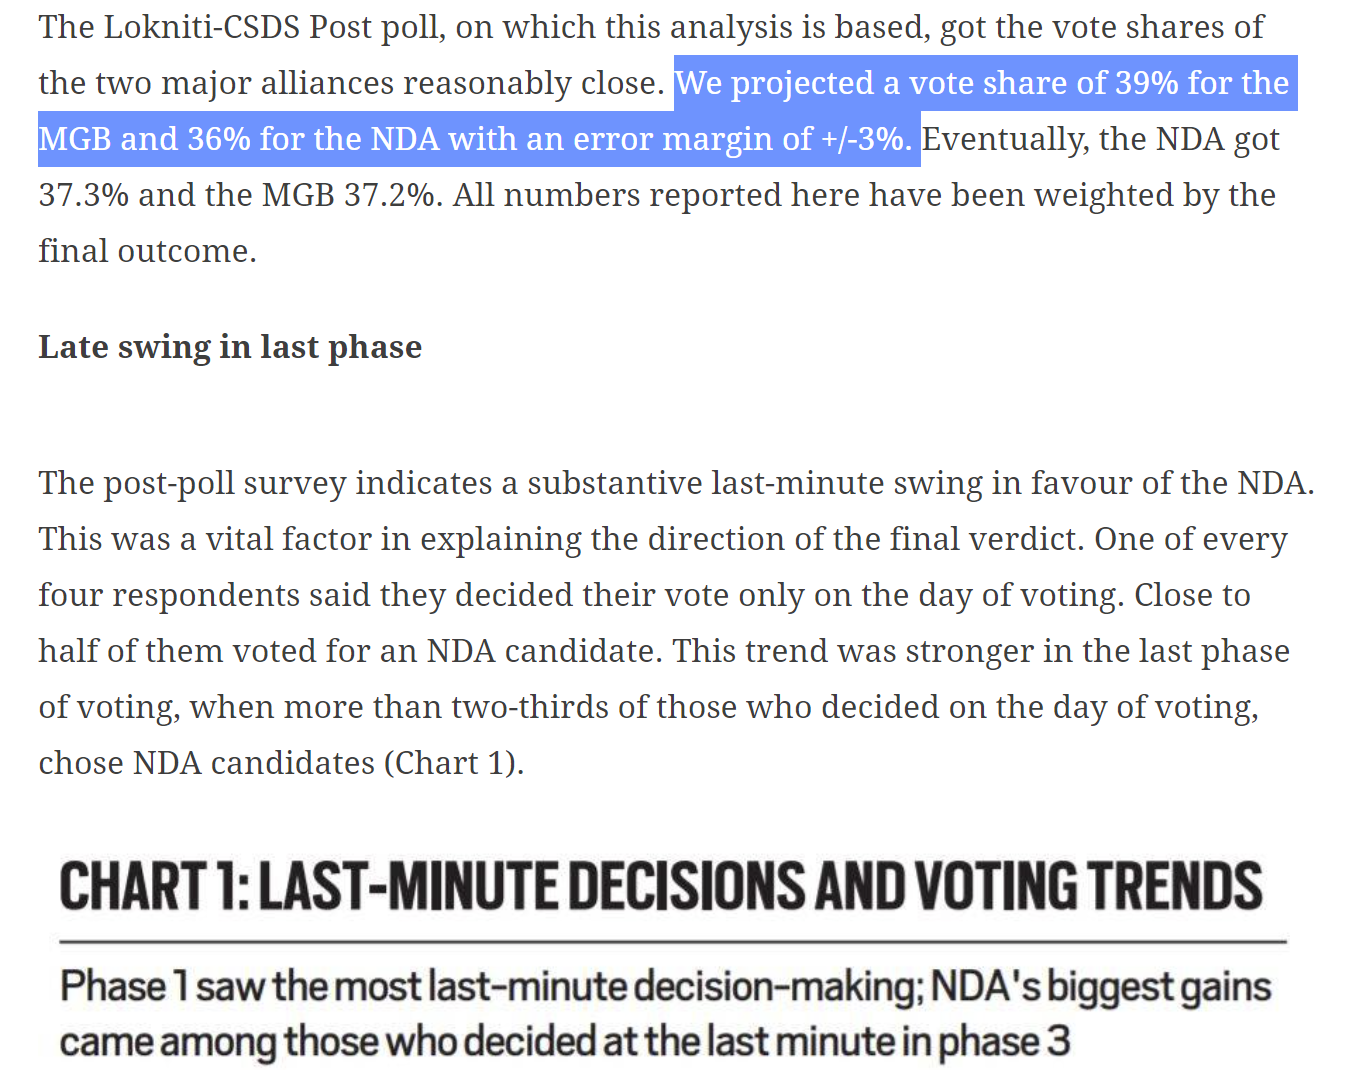
\includegraphics[width=0.95\textwidth]{graphs/l05f01.png}
\end{center}
\end{frame}
%%%%%%%%%%%%%%%%%%%%%%%%%%%%%%%%%%%

%%%%%%%%%%%%%%%%%%%%%%%%%%%%%%%%%%%
\begin{frame}
\frametitle{Margin of error}

\begin{center}
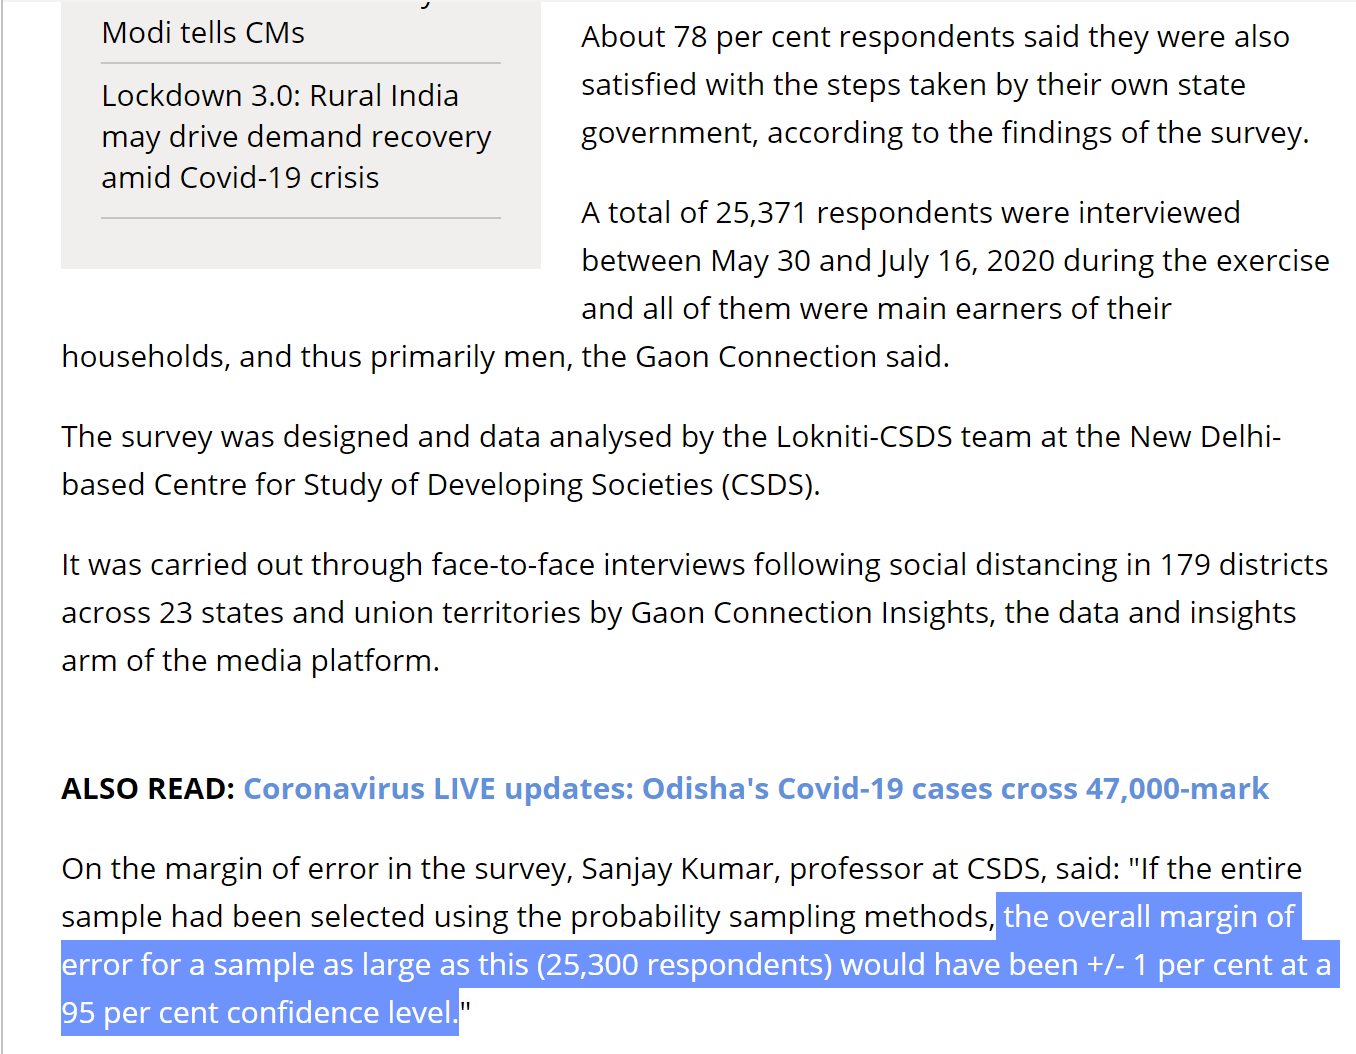
\includegraphics[width=0.5\textwidth]{graphs/l05f02.png}
\end{center}

\begin{itemize}
\item 78\% $\pm$ 1\%: We are 95\% confident that 77\% to 79\% of the public believe that the effort made by their respective state governments in curbing the coronavirus has been satisfactory.
\end{itemize}
\end{frame}

%%%%%%%%%%%%%%%%%%%%%%%%%%%%%%%%%%%

\subsection{Application exercise}

%%%%%%%%%%%%%%%%%%%%%%%%%%%%%%%%%%%


%%%%%%%%%%%%%%%%%%%%%%%%%%%%%%%%%%%
\begin{frame}{Application}

\begin{center}
\large
Run lines \color{blue}{1-26} in \color{green}{\texttt{R}}
\end{center}

\end{frame}

%%%%%%%%%%%%%%%%%%%%%%%%%%%%%%%%%%
\begin{frame}{Sampling Distribution}

Suppose you were to repeat this process many times and obtain many $\hat{p}$s. This distribution is called a \hl{sampling distribution}.

\begin{center}
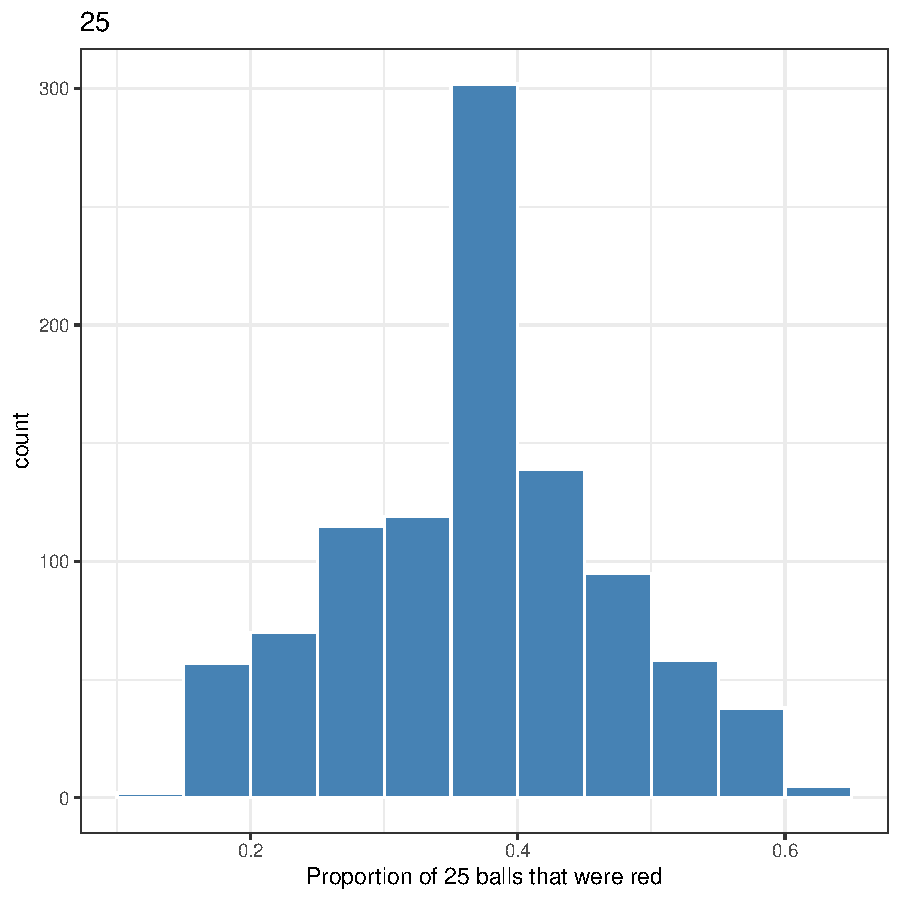
\includegraphics[width=0.45\textwidth]{graphs/l05f03.pdf}
\end{center}

\end{frame}
%%%%%%%%%%%%%%%%%%%%%%%%%%%%%%%%%%%

\begin{frame}

\dq{What is the shape and center of this distribution? Based on this distribution, what do you think is the true population proportion?}

\begin{center}
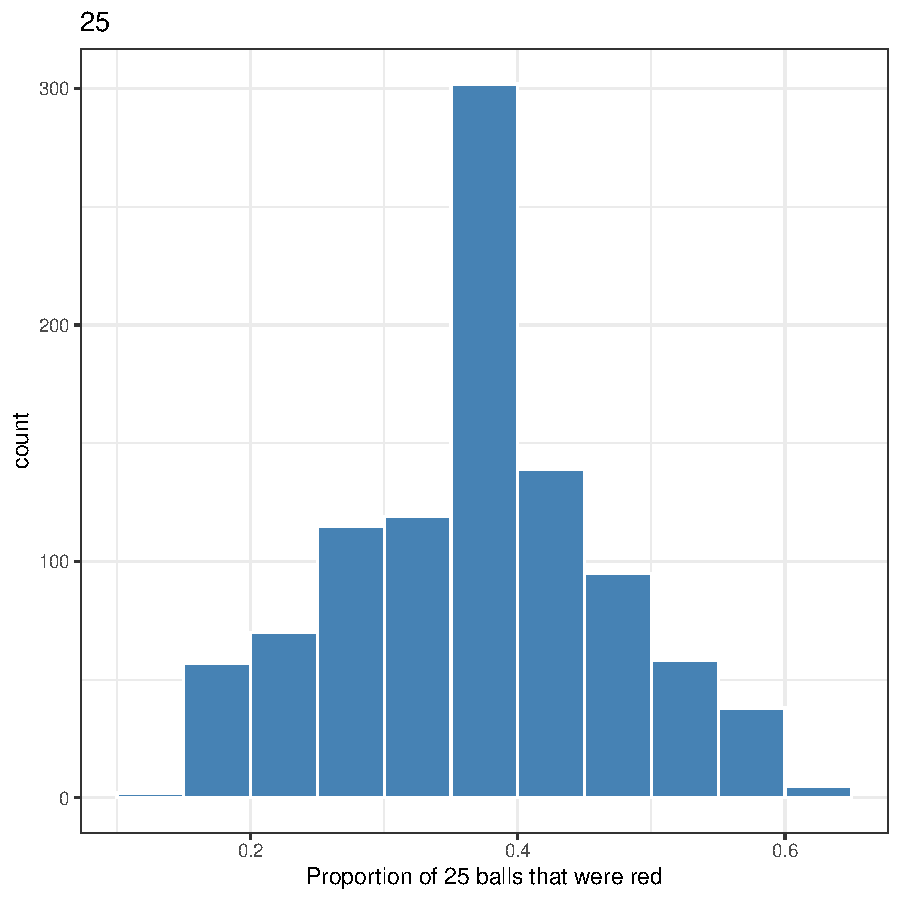
\includegraphics[width=0.35\textwidth]{graphs/l05f03.pdf}
\end{center}

$\:$ \\
\soln{\only<2>{
The distribution is unimodal and roughly symmetric. A reasonable guess for the true population proportion is the center of this distribution, approximately 0.375.
}}

\end{frame}

%%%%%%%%%%%%%%%%%%%%%%%%%%%%%%%%

\begin{frame}
\frametitle{Sampling distributions are never observed}

\begin{itemize}

\item In real-world applications, we never actually observe the sampling distribution, yet it is useful to always think of a point estimate as coming from such a hypothetical distribution.

\item Understanding the sampling distribution will help us characterize and make sense of the point estimates that we do observe.

\end{itemize}

\end{frame}

%%%%%%%%%%%%%%%%%%%%%%%%%%%%%%%%

\subsection{Central Limit Theorem}

%%%%%%%%%%%%%%%%%%%%%%%%%%%%%%%%%%

\begin{frame}
\frametitle{Central Limit Theorem}

\formula{Central limit theorem}
{Sample proportions will be nearly normally distributed with mean equal to the population proportion, $p$, and standard error equal to $\sqrt{\frac{p~(1-p)}{n}}$.
\[ \hat{p} \sim N \pr{ mean = p, SE = \sqrt{\frac{p~(1-p)}{n}} } \]
}

\begin{itemize}

\item It wasn't a coincidence that the sampling distribution we saw earlier was symmetric, and centered at the true population proportion.

\item We won't go through a detailed proof of why $SE =  \sqrt{\frac{p~(1-p)}{n}}$, but note that as $n$ increases $SE$ decreases.
\begin{itemize}
\item As $n$ increases samples will yield more consistent $\hat{p}$s, i.e. variability among $\hat{p}$s will be lower.
\end{itemize}

\end{itemize}

\end{frame}

%%%%%%%%%%%%%%%%%%%%%%%%%%%%%%%%%%%%

\begin{frame}
\frametitle{CLT - conditions}

Certain conditions must be met for the CLT to apply:

\begin{enumerate}

\item \hlGr{Independence:} Sampled observations must be independent. \\

This is difficult to verify, but is more likely if
\begin{itemize}
\item random sampling/assignment is used, and
\item if sampling without replacement, $n$ $<$ 10\% of the population.
\end{itemize}

\pause

\item \hlGr{Sample size:} There should be at least 10 expected successes and 10 expected failures in the observed sample.

This is difficult to verify if you don't know the population proportion (or can't assume a value for it). In those cases we look for the number of observed successes and failures to be at least 10.

\end{enumerate}

\end{frame}
%%%%%%%%%%%%%%%%%%%%%%%%%%%%%%%%%%


\subsection{Applying the Central Limit Theorem to a real-world setting}

%%%%%%%%%%%%%%%%%%%%%%%%%%%%%%%%%%

\begin{frame}
\frametitle{When $p$ is unknown}

\begin{itemize}

\item The CLT states $SE = \sqrt{\frac{p~(1-p)}{n}}$, with the condition that $np$ and $n(1-p)$ are at least 10, however we often don't know the value of $p$, the population proportion

\item In these cases we substitute $\hat{p}$ for $p$

\end{itemize}

\end{frame}

%%%%%%%%%%%%%%%%%%%%%%%%%%%%%%%%%%%s

\subsection{More details regarding the Central Limit Theorem}

%%%%%%%%%%%%%%%%%%%%%%%%%%%%%%%%%%%%

%%%%%%%%%%%%%%%%%%%%%%%%%%%%%%%%%%%%

\begin{frame}
\frametitle{When $p$ is low}

\dq{Suppose we have a population where the true population proportion is $p = 0.05$, and we take random samples of size $n = 50$ from this population. We calculate the sample proportion in each sample and plot these proportions. Would you expect this distribution to be nearly normal? Why, or why not?}

\pause

\soln{No, the success-failure condition is not met ($50 * 0.05 = 2.5$), hence we would not expect the sampling distribution to be nearly normal.}



\end{frame}


%%%%%%%%%%%%%%%%%%%%%%%%%%%%%%%%%%%

\begin{frame}
\frametitle{When the conditions are not met...}

\begin{itemize}

\item When either $np$ or $n(1-p)$ is small, the distribution is more discrete.
\item When $np$ or $n(1-p)$ $<$ 10, the distribution is more skewed.
\item The larger both $np$ and $n(1-p)$, the more normal the distribution.
\item When $np$ and $n(1-p)$ are both very large, the discreteness of the distribution is hardly evident, and the distribution looks much more like a normal distribution.

\end{itemize}

\end{frame}

%%%%%%%%%%%%%%%%%%%%%%%%%%%%%%%%%%%%

\subsection{Extending the framework for other statistics}

%%%%%%%%%%%%%%%%%%%%%%%%%%%%%%%%%%%%

\begin{frame}
\frametitle{Extending the framework for other statistics}

\begin{itemize}

\item The strategy of using a sample statistic to estimate a parameter is quite common, and it's a strategy that we can apply to other statistics besides a proportion.

\begin{itemize}
\item Take a random sample of students at a college and ask them how many extracurricular activities they are involved in to estimate the average number of extra curricular activities all students in this college are interested in.
\end{itemize}

\item The principles and general ideas are from this chapter apply to other parameters as well, even if the details change a little. 

\end{itemize}

\end{frame}

%%%%%%%%%%%%%%%%%%%%%%%%%%%%%%%%%%%%

\section{Confidence intervals for a proportion}

%%%%%%%%%%%%%%%%%%%%%%%%%%%%%%%%%%%%

\subsection{Capturing the population parameter}

%%%%%%%%%%%%%%%%%%%%%%%%%%%%%%%%%%%%

\begin{frame}[shrink]
\frametitle{Confidence intervals}

\begin{itemize}

\item A plausible range of values for the population parameter is called a \hl{confidence interval}.

\item Using only a sample statistic to estimate a parameter is like fishing in a murky lake with a spear, and using a confidence interval is like fishing with a net.
$\:$ \\
$\:$ \\
\begin{columns}[c]
\column{0.25\textwidth}

\includegraphics[width=\textwidth]{graphs/spear}
\column{0.5\textwidth}
{\small
We can throw a spear where we saw a fish but we will probably miss. If we toss a net in that area, we have a good chance of catching the fish.
}
\column{0.25\textwidth}

\includegraphics[width=\textwidth]{graphs/net}
\end{columns}
$\:$ \\
\item If we report a point estimate, we probably won't hit the exact population parameter. If we report a range of plausible values we have a good shot at capturing the parameter. 

\end{itemize}

{\tiny Photos by Mark Fischer (http://www.flickr.com/photos/fischerfotos/7439791462) and Chris Penny (http://www.flickr.com/photos/clearlydived/7029109617) on Flickr.}

% spear fig: http://www.flickr.com/photos/clearlydived/7029109617/sizes/q/
% net fig: http://www.flickr.com/photos/fischerfotos/7439791462/sizes/q/

\end{frame}

%%%%%%%%%%%%%%%%%%%%%%%%%%%%%%%%%%%%

\subsection{Constructing a 95\% confidence interval}

%%%%%%%%%%%%%%%%%%%%%%%%%%%%%%%%%%%%

\begin{frame}
\frametitle{Most preferred social media platform}

\dq{A recent survey of around 1100 young Indians reports Instagram as their most preferred social media platform. Estimate the true proportion of young people whose first choice is Instagram.}

\ct{\webURL{https://www.business-standard.com/article/technology/instagram-most-preferred-platform-among-indian-youth-survey-120100900588_1.html/}}

\end{frame}

%%%%%%%%%%%%%%%%%%%%%%%%%%%%%%%%%%%%

\begin{frame}
\frametitle{Most preferred social media platform}

\[ \hat{p} = 0.7 \qquad n = 1100 \]

\pause

The approximate 95\% confidence interval is defined as 
\[ point~estimate \pm 1.96 \times SE \]

\pause

\vspace{-0.25cm}
\[ SE = \sqrt{\frac{p(1-p)}{n}} = \sqrt{\frac{0.7 \times 0.3}{1100}} \approx 0.014 \]

\pause

\vspace{-0.25cm}
\begin{eqnarray*}
\hat{p} \pm 1.96 \times SE &=& 0.7 \pm 1.96 \times 0.013 \\
\pause
&=& (0.7 - 0.03, 0.7 + 0.03) \\
\pause
&=& (0.67, 0.73)
\end{eqnarray*}


\end{frame}

%%%%%%%%%%%%%%%%%%%%%%%%%%%%%%%%%%%


\begin{frame}
\frametitle{What does 95\% confident mean?}

\begin{itemize}

\item Suppose we took many samples and built a confidence interval from each sample using the equation $point~estimate \pm 1.96 \times SE$.

\item Then about 95\% of those intervals would contain the true population proportion ($p$). 

\end{itemize}

\end{frame}

%%%%%%%%%%%%%%%%%%%%%%%%%%%%%%%%%%%

\begin{frame}
\frametitle{Width of an interval}

\dq{If we want to be more certain that we capture the population parameter, i.e. increase our confidence level, should we use a wider interval or a smaller interval?}

\pause

\soln{A wider interval.}

$\:$ \\

\pause

\dq{Can you see any drawbacks to using a wider interval?}
\begin{center}

\includegraphics[width=0.9\textwidth]{graphs/garfield}
\end{center}

\pause

\soln{If the interval is too wide it may not be very informative.}

{\scriptsize Image source: http://web.as.uky.edu/statistics/users/earo227/misc/garfield\_weather.gif}

\end{frame}

%%%%%%%%%%%%%%%%%%%%%%%%%%%%%%%%%%%
%%%%%%%%%%%%%%%%%%%%%%%%%%%%%%%%%%%

\subsection{Changing the confidence level}

%%%%%%%%%%%%%%%%%%%%%%%%%%%%%%%%%%%

\begin{frame}
\frametitle{Changing the confidence level}

\[ point~estimate\pm z^\star \times SE \] 

\begin{itemize}

\item In a confidence interval, $z^\star \times SE$ is called the \hl{margin of error}, and for a given sample, the margin of error changes as the confidence level changes.

\item In order to change the confidence level we need to adjust $z^\star$ in the above formula.

\item Commonly used confidence levels in practice are 90\%, 95\%, 98\%, and 99\%.

\item For a 95\% confidence interval, $z^\star = 1.96$.

\item However, using the standard normal ($z$) distribution, it is possible to find the appropriate $z^\star$ for any confidence level.

\end{itemize}

\end{frame}

%%%%%%%%%%%%%%%%%%%%%%%%%%%%%%%%%%%%

\begin{frame}

\pq{Which of the below Z scores is the appropriate $z^\star$ when calculating a 98\% confidence interval?}

\begin{multicols}{2}
\begin{enumerate}[(a)]
\item $Z = 2.05$
\item $Z = 1.96$
\solnMult{$Z = 2.33$}
\item $Z = -2.33$
\item $Z = -1.65$
\item[]
\end{enumerate}
\end{multicols}

\soln{\only<2>{
\begin{center}
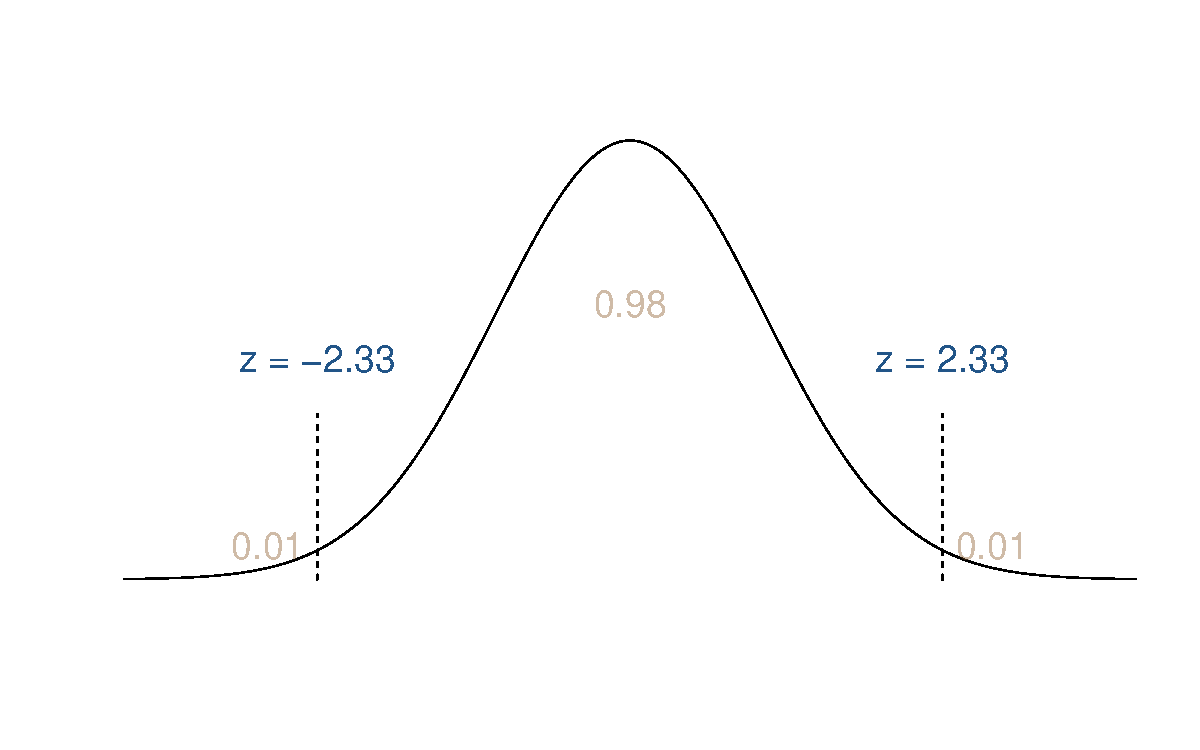
\includegraphics[width=0.5\textwidth]{graphs/l05f04}
\end{center}
}}

\end{frame}

%%%%%%%%%%%%%%%%%%%%%%%%%%%%%%%%%%%

\subsection{Interpreting confidence intervals}

%%%%%%%%%%%%%%%%%%%%%%%%%%%%%%%%%%%

\begin{frame}
\frametitle{Interpreting confidence intervals}

Confidence intervals are ...

\begin{itemize}

\item always about the population

\item not probability statements 

\item only about population parameters, not individual observations

\item only reliable if the sample statistic they're based on is an unbiased estimator of the population parameter

\end{itemize}

\end{frame}

%%%%%%%%%%%%%%%%%%%%%%%%%%%%%%%%%%%%

\section{Hypothesis testing for a proportion}

%%%%%%%%%%%%%%%%%%%%%%%%%%%%%%%%%%%%

\subsection{Hypothesis testing framework}

%%%%%%%%%%%%%%%%%%%%%%%%%%%%%%%%%%%%

\begin{frame}
\frametitle{Remember when...}

Gender discrimination experiment:

{\footnotesize
\begin{tabular}{ll  cc c} 
  		&				& \multicolumn{2}{c}{\textit{Callback}} \\
\cline{3-4}
							&			& No	& Yes 	& Total	\\
\cline{2-5}
\multirow{2}{*}{\textit{Race	}}	& Black 		& 2278	 	& 157		& 2435 	\\
							& White		& 2200	 	& 235 	 	& 2435 \\
\cline{2-5}
							&Total		& 4478		& 392		& 4870 \\
\end{tabular}
}

\pause

\[ \hat{p}_{black} \approx 0.03 ~ \text{ and } ~ \hat{p}_{white} \approx 0.05 \]

\pause

Possible explanations:
\begin{itemize}
\item Callback and race are \hl{independent}, no racial discrimination, observed difference in proportions is simply due to chance. $\rightarrow$ \orange{null} - {\small (nothing is going on)}
\item Callback and race are \hl{dependent}, there is racial discrimination, observed difference in proportions is not due to chance. $\rightarrow$ \orange{alternative} - {\small (something is going on)}

\end{itemize}

\end{frame}


%%%%%%%%%%%%%%%%%%%%%%%%%%%%%%%%%%%%

\begin{frame}
\frametitle{Result}

\begin{center}
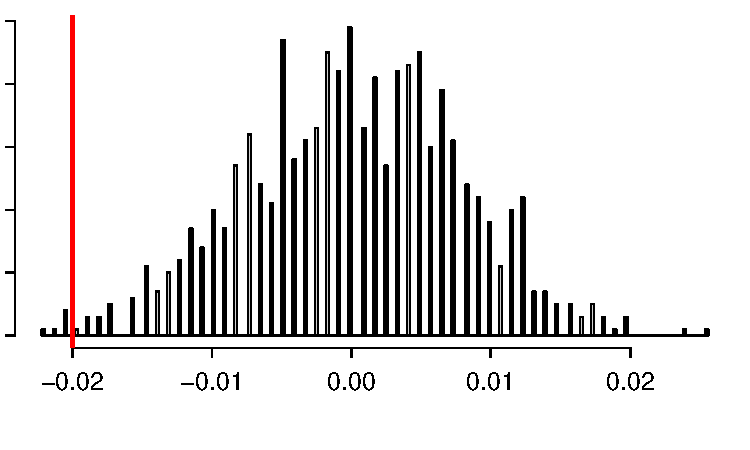
\includegraphics[width=0.5\textwidth]{graphs/l05f05}
\end{center}

\pause

Since it was quite unlikely to obtain results like the actual data or something more extreme in the simulations (callback for the African-American sounding-names 2\% or lower than those for White sounding names), we decided to reject the null hypothesis in favor of the alternative.

\end{frame}

%%%%%%%%%%%%%%%%%%%%%%%%%%%%%%%%%%%%

\begin{frame}
\frametitle{Recap: hypothesis testing framework}

\begin{itemize}
\item We start with a \hl{null hypothesis ($H_0$)} that represents the status quo.
\pause
\item We also have an \hl{alternative hypothesis ($H_A$)} that represents our research question, i.e. what we're testing for.
\pause
\item We conduct a hypothesis test under the assumption that the null hypothesis is true, either via simulation or traditional methods based on the central limit theorem (coming up next...).
\pause
\item If the test results suggest that the data do not provide convincing evidence for the alternative hypothesis, we stick with the null hypothesis. If they do, then we reject the null hypothesis in favor of the alternative.
\end{itemize}
\pause
We'll formally introduce the hypothesis testing framework using an example on testing a claim about a proportion.

\end{frame}

%%%%%%%%%%%%%%%%%%%%%%%%%%%%%%%%%%%%
 
\begin{frame}
\frametitle{Decision errors (cont.)}

There are two competing hypotheses: the null and the alternative. In a hypothesis test, we make a decision about which might be true, but our choice might be incorrect. \\

\pause

\begin{center}
\begin{tabular}{l l | c c}
\multicolumn{2}{c}{} & \multicolumn{2}{c}{\textbf{Decision}} \\
& & fail to reject $H_0$ &  reject $H_0$ \\
  \cline{2-4}
& $H_0$ true & \onslide<3->{\green{$\checkmark$}} &  \onslide<5->{\orange{Type 1 Error}} \\
\raisebox{1.5ex}{\textbf{Truth}} & $H_A$ true & \onslide<6->{\orange{Type 2 Error}} & \onslide<4->{\green{$\checkmark$}} \\
  \cline{2-4}
\end{tabular}
\end{center}

\begin{itemize}
\item \onslide<5->{A \hl{Type 1 Error} is rejecting the null hypothesis when $H_0$ is true.}

\item \onslide<6->{A \hl{Type 2 Error} is failing to reject the null hypothesis when $H_A$ is true.}

\item \onslide<7->{We (almost) never know if $H_0$ or $H_A$ is true, but we need to consider all possibilities.}

\end{itemize}

\end{frame}

%%%%%%%%%%%%%%%%%%%%%%%%%%%%%%%%%%%%

\begin{frame}[shrink]
\frametitle{Hypothesis Test as a trial}

If we think of a hypothesis test as a criminal trial then it makes sense to frame the verdict in terms of the null and alternative hypotheses:
\begin{align*}
H_0&:\text{ Defendant is innocent} \\
H_A&:\text{ Defendant is guilty}
\end{align*}

Which type of error is being committed in the following circumstances?

\begin{itemize}
\item Declaring the defendant innocent when they are actually guilty
\soln{\only<2->{\begin{center}\hl{Type 2 error}\end{center}}}
\item Declaring the defendant guilty when they are actually innocent
\soln{\only<3->{\begin{center}\hl{Type 1 error}\end{center}}}
\end{itemize}

\only<4->{Which error do you think is the worse error to make?}
\end{frame}

%%%%%%%%%%%%%%%%%%%%%%%%%%%%%%%%%%%%

\begin{frame}
\frametitle{Type 1 error rate}

\begin{itemize}

\item As a general rule we reject $H_0$ when the p-value is less than 0.05, i.e. we use a \hl{significance level} of 0.05, \mathhl{\alpha = 0.05}.

\pause

\item This means that, for those cases where $H_0$ is actually true, we do not want to incorrectly reject it more than 5\% of those times. 

\pause

\item In other words, when using a 5\% significance level there is about 5\% chance of making a Type 1 error if the null hypothesis is true.
\[ \mathhl{ P(\text{Type 1 error} \: | \: \text{$H_0$ true}) = \alpha } \]

\pause

\item This is why we prefer small values of $\alpha$ -- increasing $\alpha$ increases the Type 1 error rate.

\end{itemize}

\end{frame}

%%%%%%%%%%%%%%%%%%%%%%%%%%%%%%%%%%%%

\subsection{Formal testing using p-values}

%%%%%%%%%%%%%%%%%%%%%%%%%%%%%%%%%%%%

\begin{frame}
\frametitle{Example}

\begin{center}
\large
Lines \color{blue}{174-193} in \color{green}{R}
\end{center}
\end{frame}
 
%%%%%%%%%%%%%%%%%%%%%%%%%%%%%%%%%%

\begin{frame}
\frametitle{Setting the hypotheses}

\begin{itemize}

\item The \hl{parameter of interest} is the proportion of red balls.

\pause

\item There may be two explanations why our sample proportion is lower than 0.375.
\begin{itemize}
\item The true population proportion is different than 0.375.
\item The true population mean is 0.375, and the difference between the true population proportion and the sample proportion is simply due to natural sampling variability.
\end{itemize}

 \end{itemize}

\end{frame}

%%%%%%%%%%%%%%%%%%%%%%%%%%%%%%%%%%
 
\begin{frame}
\frametitle{Setting the hypotheses}

\begin{itemize}

\item We start with the assumption that 37.5\% of balls are red.
\[ \mathhl{H_0:}~p = 0.375 \]

\pause

\item We test the claim that the proportion of red balls is different than 37.5\%
\[ \mathhl{H_A:}~p \ne 0.375 \]

\end{itemize}

\end{frame}

%%%%%%%%%%%%%%%%%%%%%%%%%%%%%%%%%


 
\begin{frame}
\frametitle{Test statistic}
 
In order to evaluate if the observed sample proportion is unusual for the hypothesized sampling distribution, we determine how many standard errors away from the null it is, which is also called the \hl{test statistic}.
 
\pause
 
\[ \hat{p} \sim N \pr{ \mu = 0.375, SE = \sqrt{\frac{0.375 \times 0.625}{50} }  } \]

\pause

\[ Z = \frac{0.3 - 0.375}{0.07} = -1.1 \]
 
 \pause
 
\dq{The sample proportion is -1.1 standard errors away from the hypothesized value. Is this considered unusually low? That is, is the result \hl{statistically significant}?}
 
\pause
 
\soln{Yes, and we can quantify how unusual it is using a p-value.}
 
\end{frame}
 
%%%%%%%%%%%%%%%%%%%%%%%%%%%%%%%%%%

\begin{frame}
\frametitle{p-values}

\begin{itemize}

\item We then use this test statistic to calculate the \hl{p-value}, the probability of observing data at least as favorable to the alternative hypothesis as our current data set, if the null hypothesis were true.

\pause

\item If the p-value is \hl{low} (lower than the significance level, $\alpha$, which is usually 5\%) we say that it would be very unlikely to observe the data if the null hypothesis were true, and hence \hl{reject $H_0$}.

\pause

\item If the p-value is \hl{high} (higher than $\alpha$) we say that it is likely to observe the data even if the null hypothesis were true, and hence \hl{do not reject $H_0$}.

\end{itemize}

\end{frame}

%%%%%%%%%%%%%%%%%%%%%%%%%%%%%%%%%%%%

\begin{frame}
\frametitle{Virtual bowl example - p-value}

\hl{p-value:} probability of observing data at least as favorable to $H_A$ as our current data set (a sample proportion lower than 0.3), if in fact $H_0$ were true (the true population proportion was 0.375).

\pause

\[ P(|Z| > 1.1) < 0.14 \]

\end{frame}

%%%%%%%%%%%%%%%%%%%%%%%%%%%%%%%%%

\begin{frame}
\frametitle{The Bowl Example}

\begin{itemize}

\item p-value $>$ 0.05

\pause


\pause
\item Since p-value is \orange{high} (higher than 5\%) we \orange{don't reject $H_0$}.


\pause
\item The difference between the null value of 0.375 and observed sample proportion of 0.3 is \orange{due to chance} or sampling variability.

\end{itemize}

\end{frame}

%%%%%%%%%%%%%%%%%%%%%%%%%%%%%%%%%%%

\subsection{Choosing a significance level}

%%%%%%%%%%%%%%%%%%%%%%%%%%%%%%%%%%%%

\begin{frame}
\frametitle{Choosing a significance level}

\begin{itemize}

\item While the the traditional level is 0.05, it is helpful to adjust the significance level based on the application. 

\item Select a level that is smaller or larger than 0.05 depending on the consequences of any conclusions reached from the test.

\item If making a Type 1 Error is dangerous or especially costly, we should choose a small significance level (e.g. 0.01). Under this scenario we want to be very cautious about rejecting the null hypothesis, so we demand very strong evidence favoring $H_A$ before we would reject $H_0$.

\item If a Type 2 Error is relatively more dangerous or much more costly than a Type 1 Error, then we should choose a higher significance level (e.g. 0.10). Here we want to be cautious about failing to reject $H_0$ when the null is actually false.

\end{itemize}

\end{frame}

%%%%%%%%%%%%%%%%%%%%%%%%%%%%%%%%%%%%
 
\subsection{One vs. two sided hypothesis tests}
 
%%%%%%%%%%%%%%%%%%%%%%%%%%%%%%%%%%%%
 
\begin{frame}
\frametitle{One vs. two sided hypothesis tests}
 
\begin{itemize}
 
\item In two sided hypothesis tests we are interested in whether $p$ is either above or below some null value $p_0$: $H_A: p \ne p_0$.
 
\item In one sided hypothesis tests we are interested in $p$ differing from the null value $p_0$ in one direction (and not the other):
\begin{itemize}
\item If there is only value in detecting if population parameter is less than $p_0$, then $H_A: p < p_0$.
\item If there is only value in detecting if population parameter is greater than $p_0$, then $H_A: p > p_0$.
\end{itemize}

\item Two-sided tests are often more appropriate as we often want to detect if the data goes clearly in the opposite direction of our alternative hypothesis as well.

\end{itemize}

\end{frame}

%%%%%%%%%%%%%%%%%%%%%%%%%%%%%%%%%%%%
 


\end{document}